\begin{frame}[t]{Direct Preference Optimization (DPO)}
  \begin{itemize}
    \item[\textcolor{red}{$\blacktriangleright$}] \textbf{Key idea:} Optimize the policy directly on preference pairs, with no reward model and no RL rollouts.
    \item[\textcolor{red}{$\blacktriangleright$}] \textbf{Reference:} Rafailov et al., 2023.
  \end{itemize}

  \vspace{0.4em}
  \textbf{DPO loss}, on the same preference triples $(x, y_w, y_l)$ used to train an RM:

  \[
  L_{\mathrm{DPO}} = -\log \frac{
      \exp\left(\beta \log \frac{\pi_\theta(y_w \mid x)}{\pi_{\text{ref}}(y_w \mid x)}\right)
    }{
      \exp\left(\beta \log \frac{\pi_\theta(y_w \mid x)}{\pi_{\text{ref}}(y_w \mid x)}\right) + \exp\left(\beta \log \frac{\pi_\theta(y_l \mid x)}{\pi_{\text{ref}}(y_l \mid x)}\right)
    }
  \]

  \footnotesize
  where $y_w$ is the preferred response, $y_l$ the dispreferred one, $\pi_\theta$ the policy being trained, $\pi_{\text{ref}}$ the frozen reference (SFT) policy, and $\beta$ controls how far $\pi_\theta$ is allowed to move away from $\pi_{\text{ref}}$.
\end{frame}

\begin{frame}[t]{Why DPO Works}
  \begin{itemize}\itemsep0.4em
    \item[\textcolor{red}{$\blacktriangleright$}] Since $\frac{e^{a}}{e^{a} + e^{b}} = \sigma(a - b)$, the loss above is the same expression written with a sigmoid:
      \[
        L_{\mathrm{DPO}} = -\log \sigma\!\left(
          \beta \log \frac{\pi_\theta(y_w \mid x)}{\pi_{\text{ref}}(y_w \mid x)}
          - \beta \log \frac{\pi_\theta(y_l \mid x)}{\pi_{\text{ref}}(y_l \mid x)}
        \right)
      \]
    \item[\textcolor{red}{$\blacktriangleright$}] Compare it with the reward-model loss $-\log\sigma\big(r_\phi(x,y_w) - r_\phi(x,y_l)\big)$: the two are identical once we read
      $\;\hat{r}_\theta(x,y) = \beta \log \frac{\pi_\theta(y \mid x)}{\pi_{\text{ref}}(y \mid x)}$ as an \emph{implicit} reward.
    \item[\textcolor{red}{$\blacktriangleright$}] The policy is therefore its own reward model, which is what the paper's title refers to. Fitting the preferences fits the policy in one step.
  \end{itemize}

  \vspace{0.3em}
  \textcolor{red}{\textbf{Benefits:}}
  \begin{itemize}
    \item Simpler and more stable than PPO: a plain supervised loss on a fixed dataset.
    \item Two networks instead of four, and no sampling loop during training.
  \end{itemize}
\end{frame}

\begin{frame}{Direct Preference Optimization (DPO)}
  \begin{figure}
    \centering
    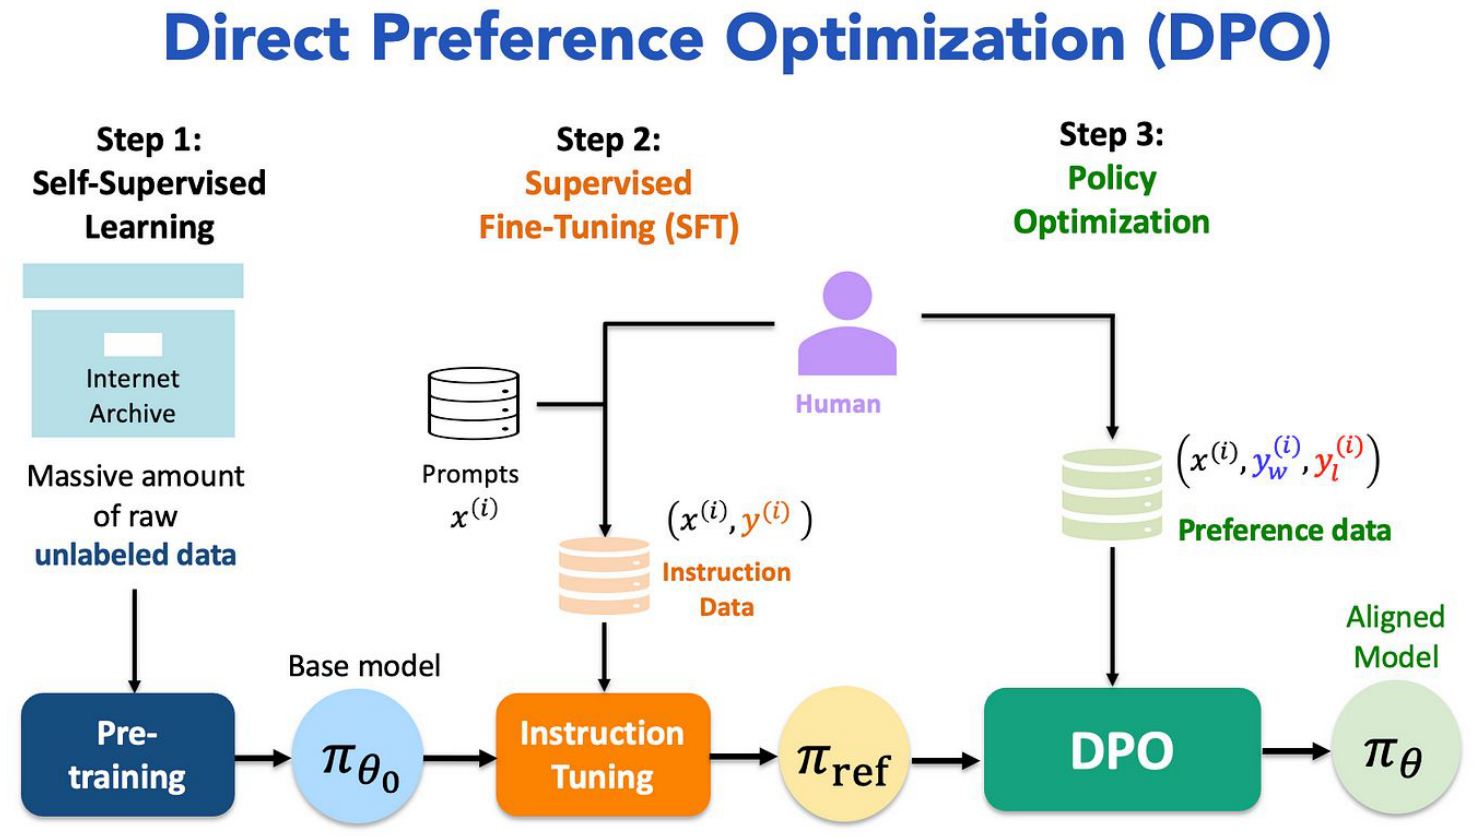
\includegraphics[width=0.74\paperwidth,height=0.60\paperheight,keepaspectratio]{images/llm-rlhf/finetune_dpo_three_steps.png}
    \caption*{\scriptsize Source: L.~M.~Po, ``Direct Preference Optimization (DPO) of LLMs: A Paradigm Shift,'' \textit{Medium}, 2024.}
  \end{figure}
\end{frame}
